\subsection*{Modello 2 - small-1202 e small-1203}

% Introduzione su strategia del training -> qual è l'obiettivo dell'esperimento?
Avendo sperimentato con i vari modelli, abbiamo iniziato a effettuare alcuni addestramenti aumentando il
numero di epoche. Si è deciso quindi di procedere con il training su tutti i parametri della rete e non
congelare alcuni layer con l'opzione \verb|freeze| ma bilanciando l'operazione optando per la dimensione
del modello più piccola quale la versione small YOLOv8s. Il numero di epoche per esecuzione è stato impostato a 120 e per tale motivo i vari modelli sono stati
nominati come \verb|small-120x|. 

Il primo dei due modelli, \verb|small-1202|, ha visto una esecuzione 
comunque non ottimale visto che alcuni dei valori di loss rispetto alla validazione non sono stati 
salvati per alcuni problemi durante l'esecuzione su colab. Ciononostante si è visto, come in figura
\ref*{fig:v2-1}, che i valori delle funzioni di loss continuavano a decrescere mentre le metriche
o rimanevano costanti, come precision e recall, o andavano a migliorare, come mAP50.

\begin{figure}[h]
    \centering
    \includegraphics[width=0.8\textwidth]{v_2/small-1202/results.png}
    \caption{Andamento funzioni di loss e metriche durante l'esecuzione di \texttt{small-1202}}
    \label{fig:v2-1}
\end{figure}

La fase di training è stata pertanto ripetuta con l'esecuzione \verb|small-1203| che rispetto al nome assegnatogli
ha avuto 300 epoche a disposizione per l'addestramento mantenendo gli stessi iperparametri del tentativo precedente.

% Dettagli configurazione, tipologia modello e iperparametri, dove è stato eseguito il train
Di seguito sono riportati tutti gli iperparametri più importanti che caratterizzano questi addestramenti:

\begin{table}[h!]
    \centering
    \begin{tabular}{lc}
        \hline
        \textbf{Iperparametro} & \textbf{Valore} \\
        \hline
        epoche & 300  \\
        optimizer & auto (SGD) \\
        learning rate (lr0) & 0.01 \\
        learning rate (lrf) & 0.01 \\
        momentum & 0.937 \\
        weight\_decay & 0.0005 \\
        imgsz & 640 \\
        dropout & 0.15 \\
        patience & 100 \\
        \midrule
        hsv\_h & 0.7 \\
        degrees & 120 \\
        shear & 55 \\
        \hline
    \end{tabular}
    \caption{Configurazione iperparametri del modello \texttt{small-1203} per il training}
    \label{tab:v2-model-configs}
    \end{table}

In particolare da notare nella tabella \ref*{tab:v2-model-configs} l'aggiunta dell'iperparametro \texttt{dropout} rispetto alla configurazione
del modello \texttt{small-1202} per poter introdurre una certa regolarizzazione all'interno della fase
di apprendimento. 
Abbiamo poi sfruttato il parametro \texttt{patience} che indica quante epoche aspettare
prima di effettuare early stopping nel caso in cui non ci fossero stati miglioramenti delle prestazioni.
% Risultati training
    % - andamento training

    \begin{figure}[!htb]
        \centering
        \includegraphics[width=0.8\textwidth]{v_2/small-1203/results.png}
        \caption{Andamento funzioni di loss e metriche durante l'esecuzione di \texttt{small-1203}}
        \label{fig:v2-2}
    \end{figure}
    % - grafici recall e precision e performance e F1
    \begin{figure}[!htb]
        \centering
        \begin{subfigure}{.5\textwidth}
            \centering
            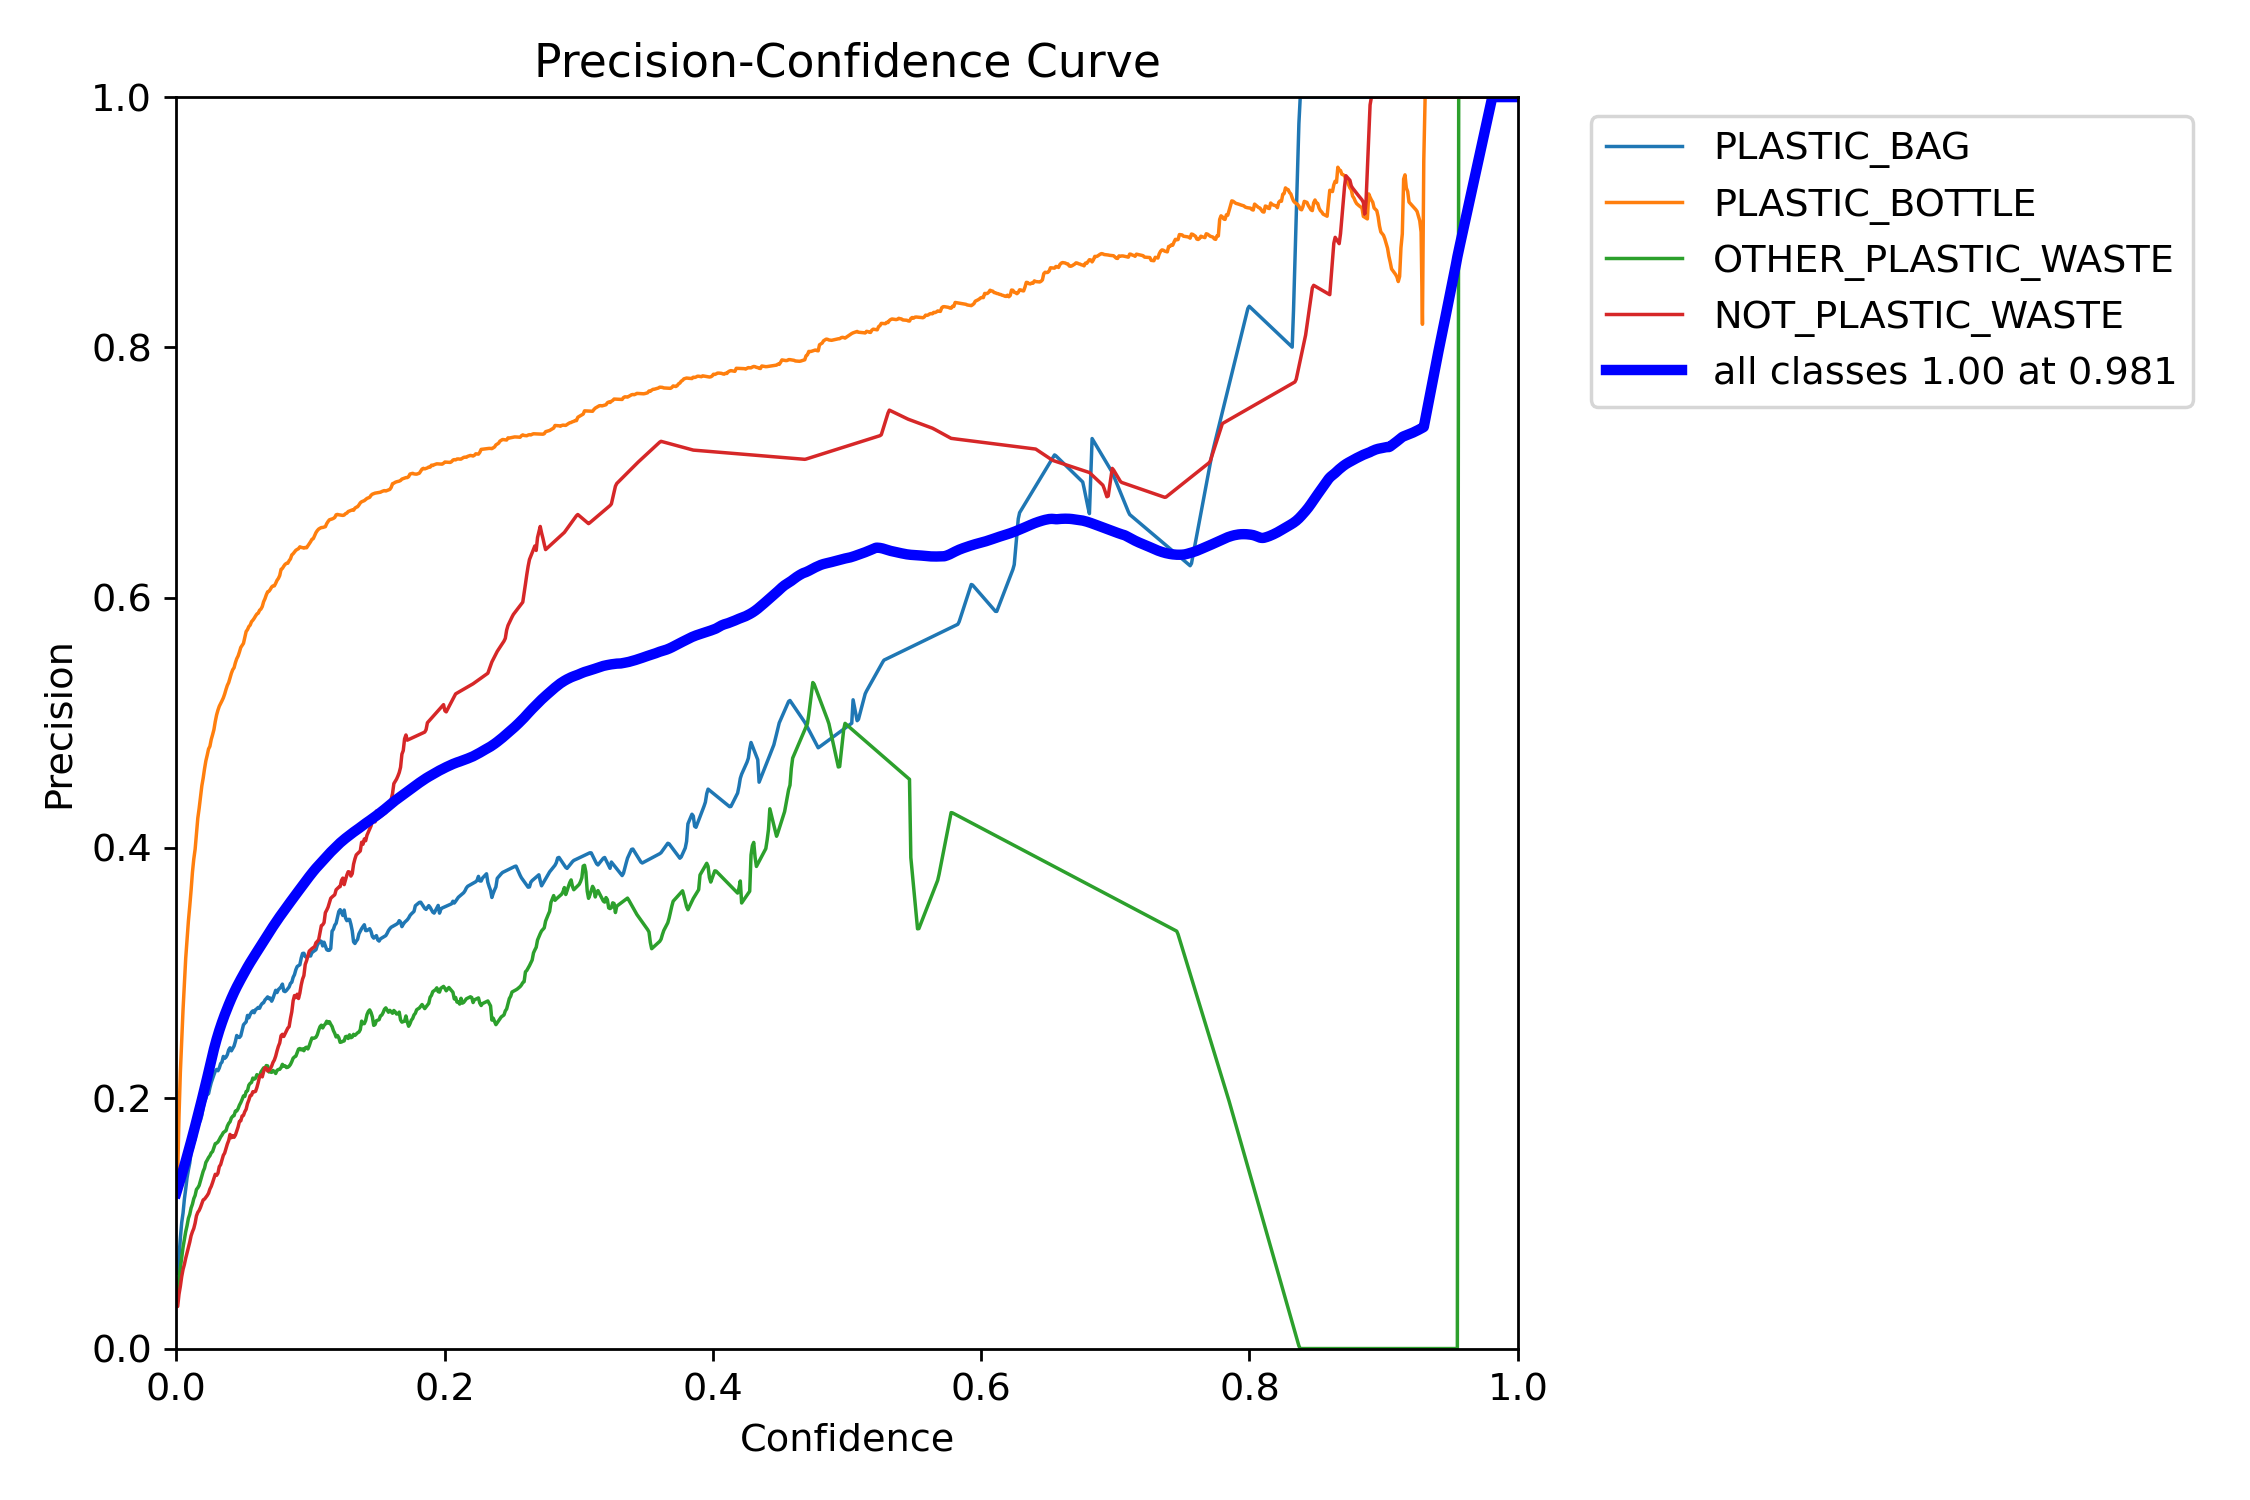
\includegraphics[width=.9\linewidth]{v_2/small-1203/P_curve.png}
            \subcaption{P-curve}
            \label{fig:v2-3.1}
          \end{subfigure}%
          \begin{subfigure}{.5\textwidth}
            \centering
            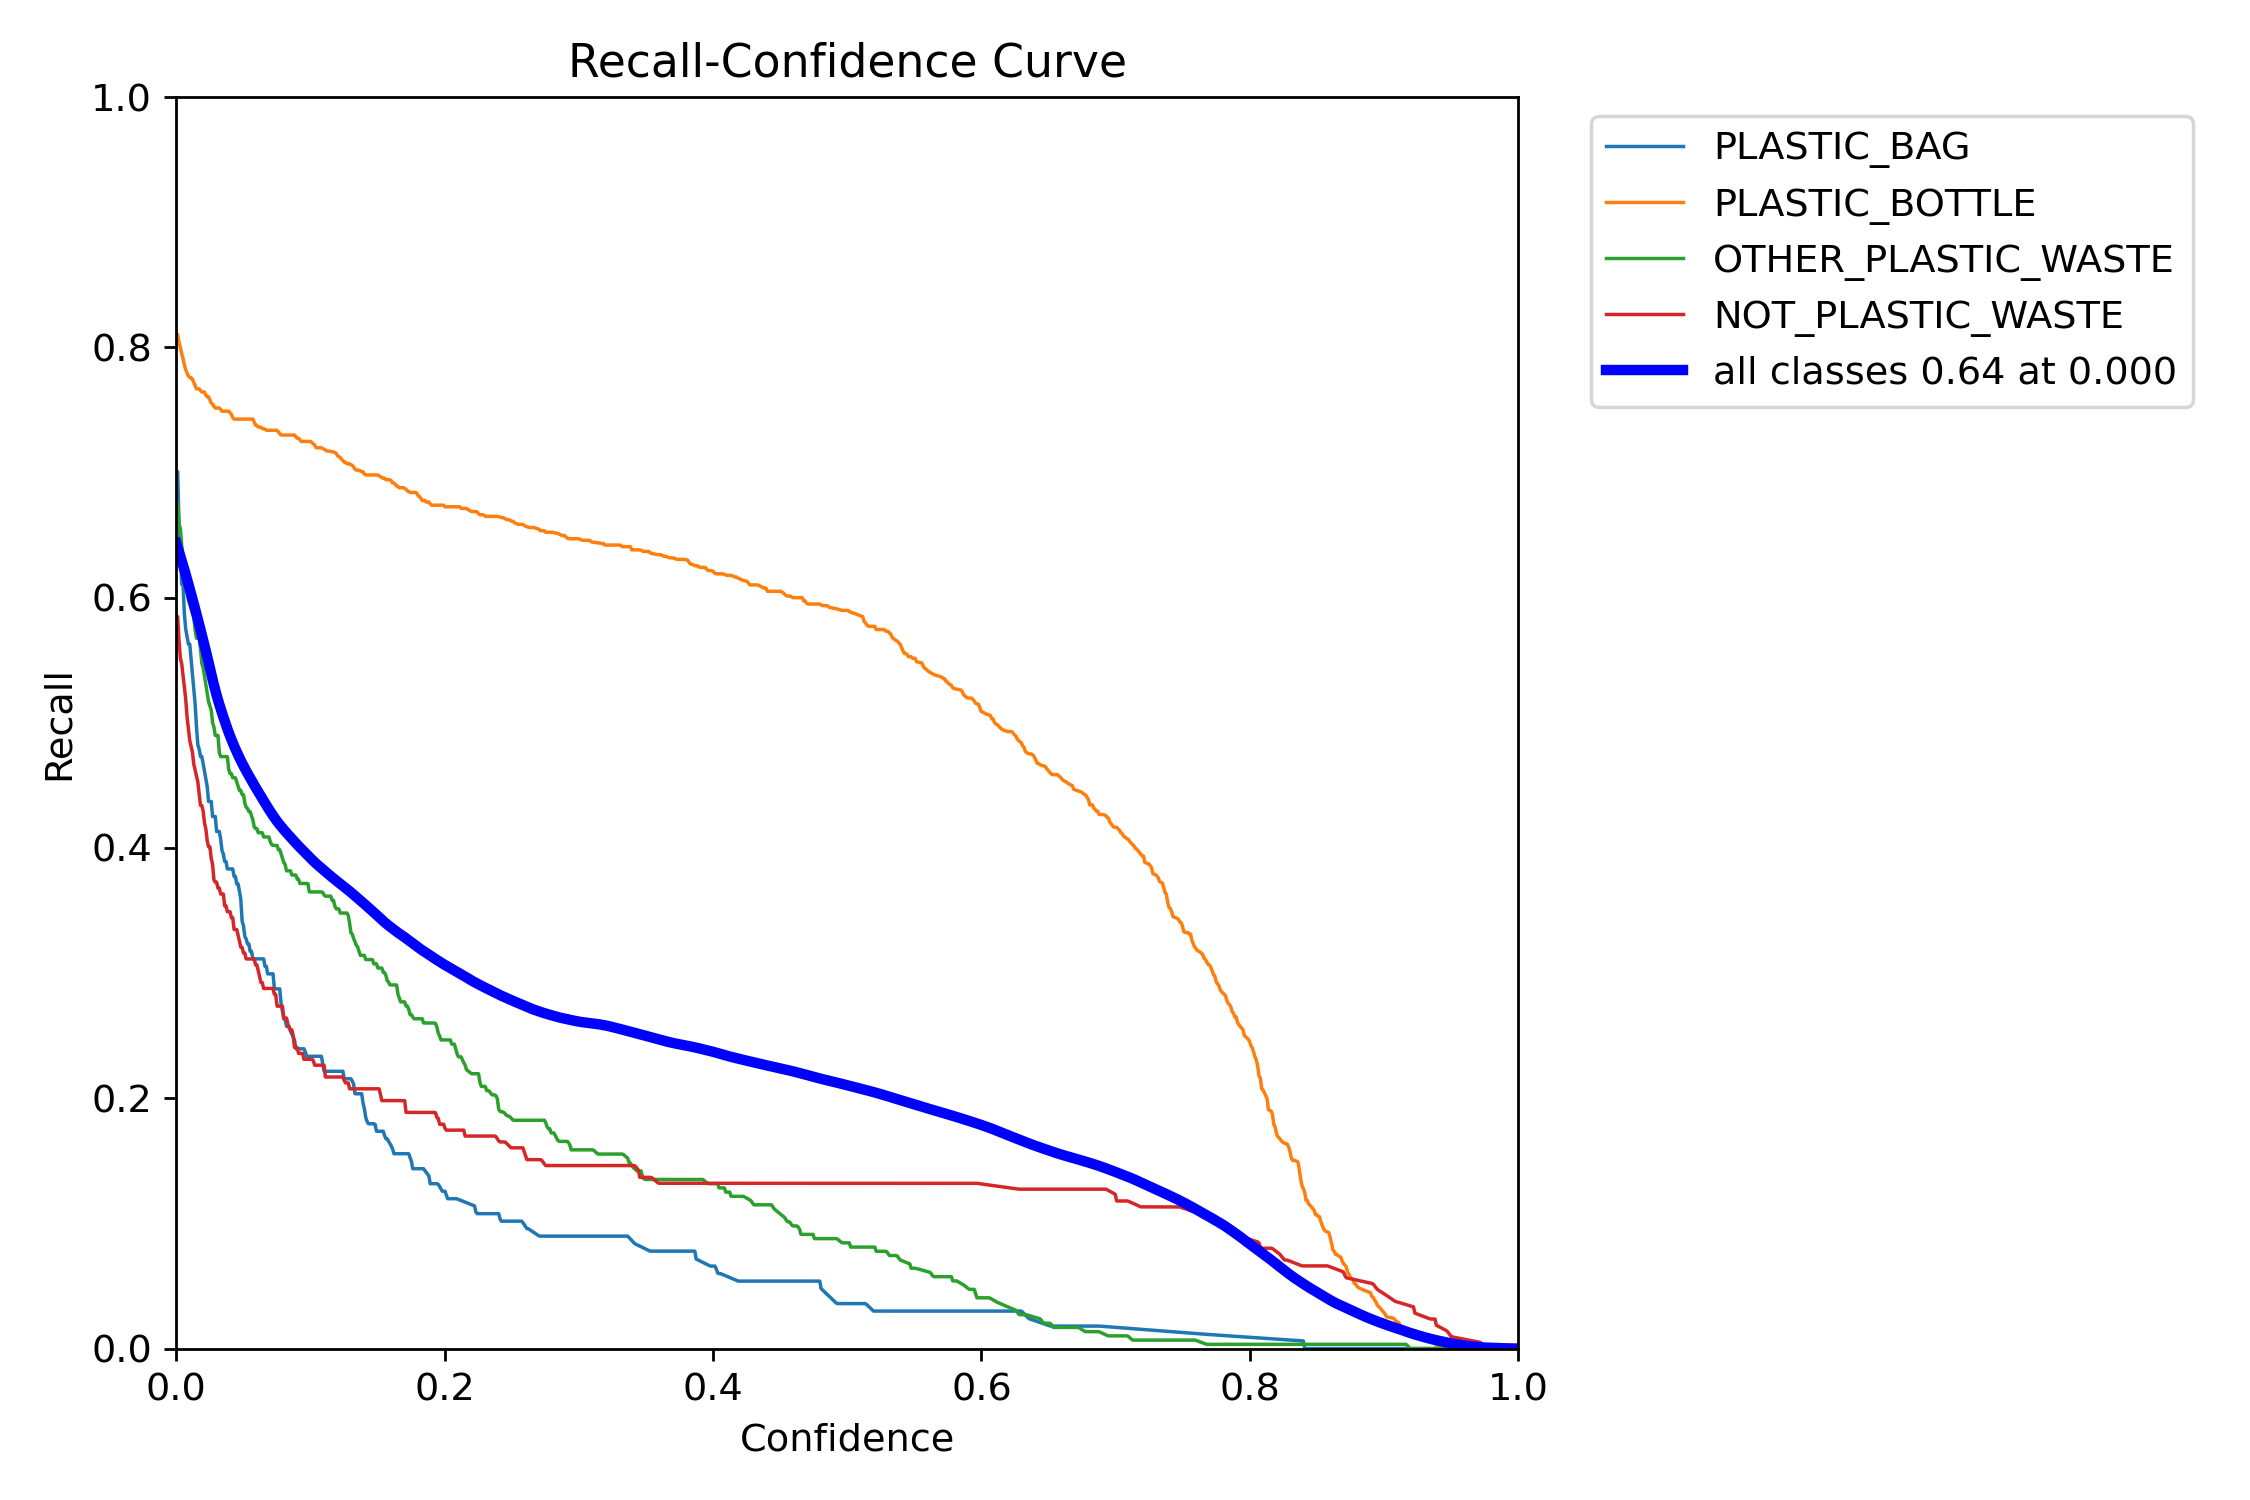
\includegraphics[width=.9\linewidth]{v_2/small-1203/R_curve.png}
            \subcaption{R-curve}
            \label{fig:v2-3.2}
          \end{subfigure}
          \vskip\baselineskip
        \begin{subfigure}{.5\textwidth}
          \centering
          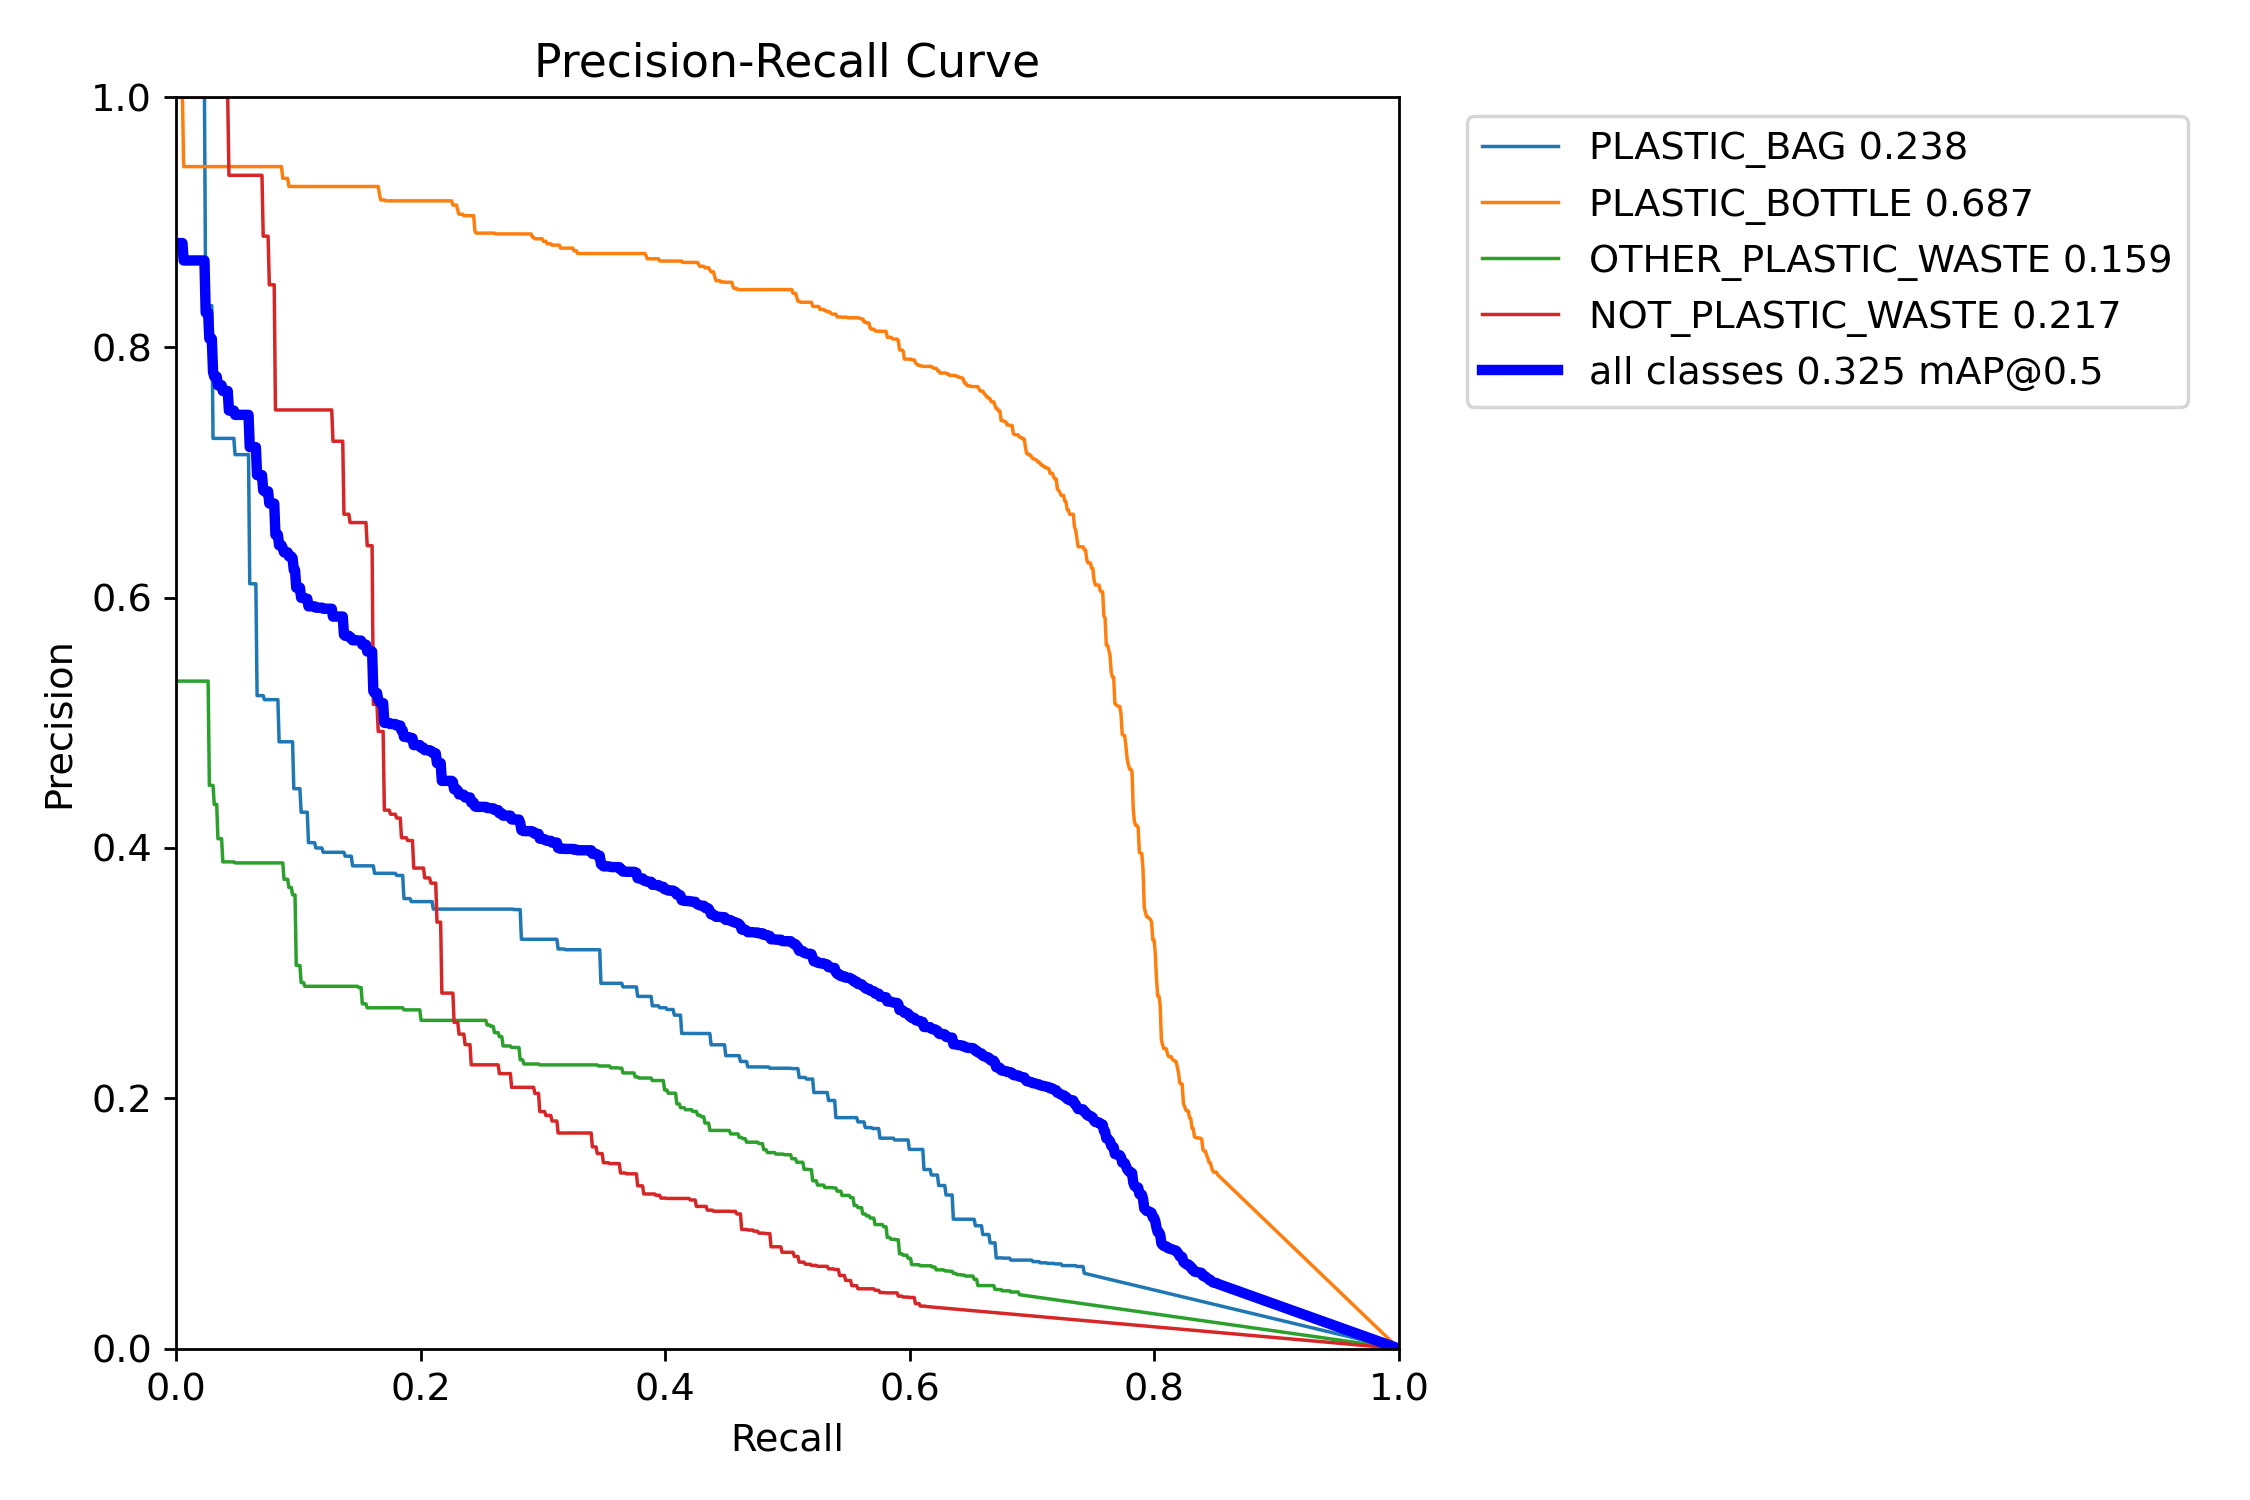
\includegraphics[width=.9\linewidth]{v_2/small-1203/PR_curve.png}
          \subcaption{PR-curve}
          \label{fig:v2-3.3}
        \end{subfigure}
        \begin{subfigure}{.49\textwidth}
            \centering
            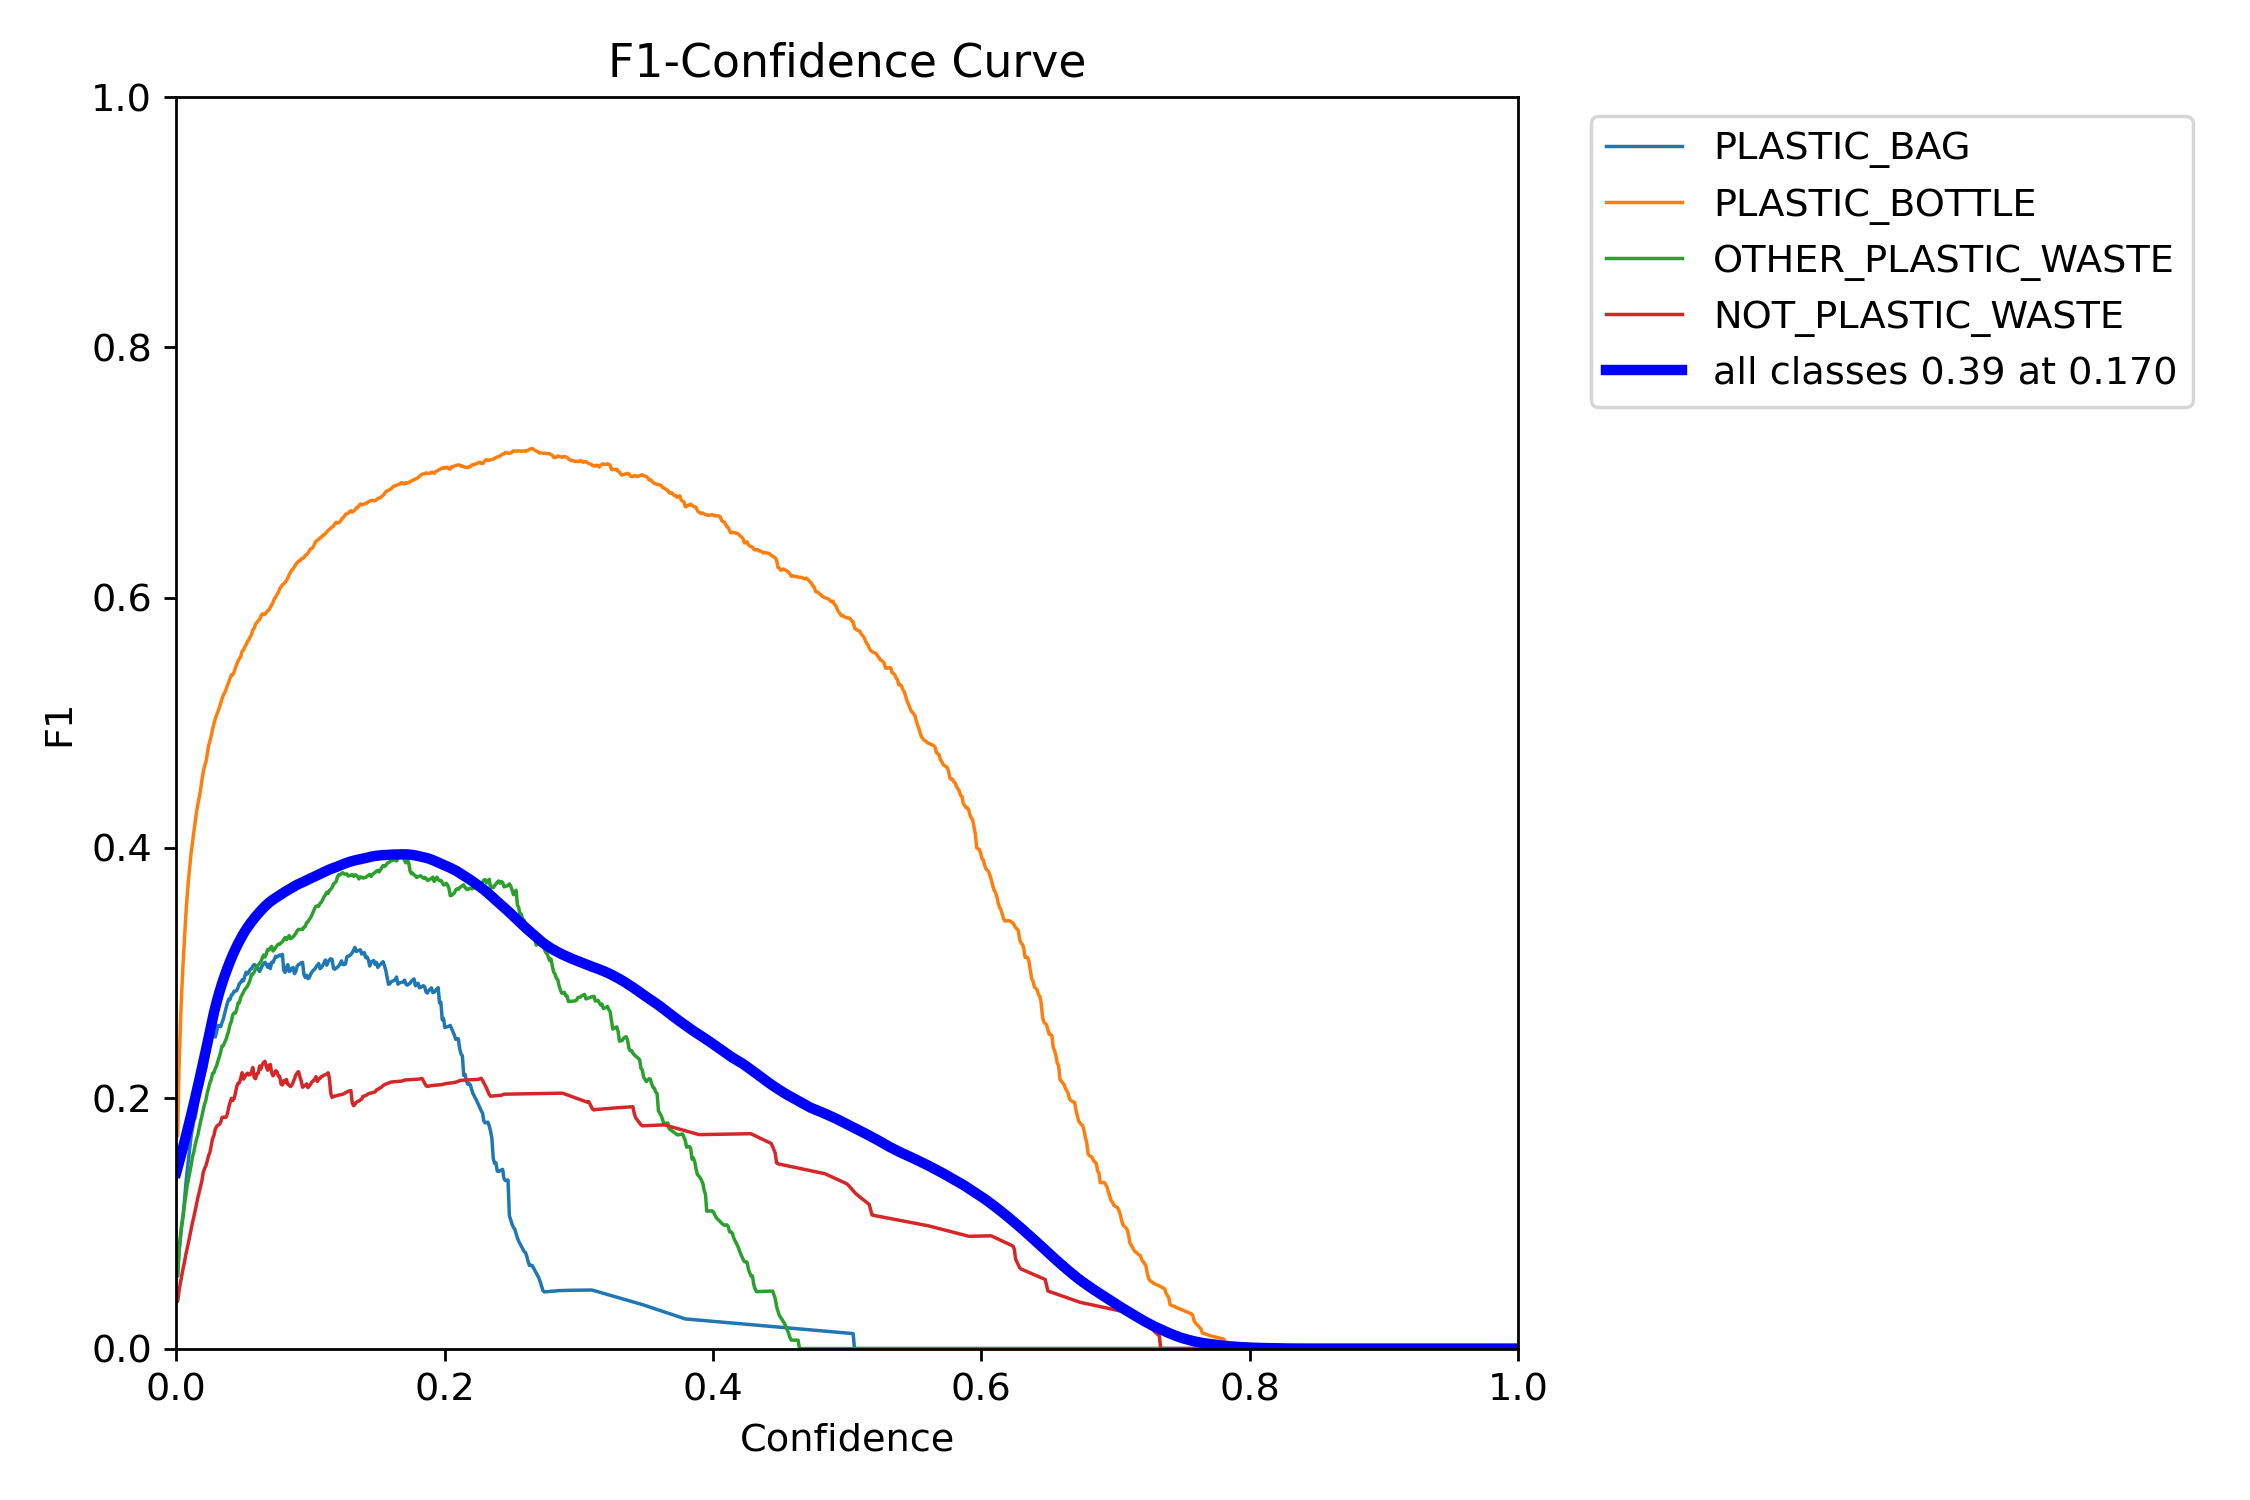
\includegraphics[width=.9\linewidth]{v_2/small-1203/F1_curve.png}
            \subcaption{F1-curve}
            \label{fig:v2-3.4}
          \end{subfigure}

        \caption{Da in alto a sinistra in poi, curva di confidenza della precisione, 
        curva di confidenza del richiamo, curva precisione-richiamo e
        curva di confidenza F1 per il modello \texttt{small-1203}}
        \label{fig:v2-3}
    \end{figure}


    % - matrici di confusione
    
    % - tabella performance test set

% Commento risultati
Quello che si è potuto vedere dai risultati e dalle performance di questi modelli, come è possibile
consultare dai grafici in figura \ref*{fig:v2-2} e in tabella \ref*{table:v2-1}, è che la rete
tende ad avere discreti precisione e richiamo ma non troppo soddisfacenti. 
In particolare se si considera una delle metriche più significative quali mAP50 vediamo che si 
raggiunge il valore nel caso migliore del 37.4\% che potrebbe essere sì considerato un risultato
accettabile ma che presenta alcuni dubbi sull'efficacia del modello. 

Considerando anche gli andamenti delle funzioni di errore durante l'addestramento (figura \ref*{fig:v2-2}) si può notare
come i valori di loss con il set di validazione vengono plafonati mentre  quelli inerenti al 
training set in genere si riducono ma avendo un comportamento oscillante. Questo può indicare
un momento di stallo che può portare a un indesiderato overfitting della rete.

È anche possibile vedere dalla tabella \ref*{table:v2-1} e dalla matrice di confusione normalizzata
in figura \ref*{fig:v2-4} come la distribuzione sbilanciata delle classi comporta sì ottimi risultati
per la classe \texttt{PLASTIC\_BOTTLE} ma risultati discreti nelle altre se non addirittura pessime
considerando la classe \texttt{OTHER\_PLASTIC\_WASTE}. Questo fenomeno si è visto in tutti gli esperimenti
e non è stato possibile rimuoverlo ma solo arginarlo in parte.

Anche per quanto riguarda l'analisi delle curve di confidenza delle varie metriche, figura \ref*{fig:v2-3},
si può notare come la classe \texttt{PLASTIC\_BOTTLE}, rappresentata dalle curve arancioni,
abbia performance nettamente migliori rispetto alla media.

Se il modello fosse pensato per il solo riconoscimento delle bottiglie di plastica probabilmente
si potevano raggiungere ottimi risultati ma di contro sarebbero stati poco utili poi all'atto 
pratico. 

\begin{table}[!htb]
    \centering
    \begin{tabularx}{\textwidth}{lYYYc}
        \toprule
        Class &  P & R & mAP50 & mAP50-95 \\
        \midrule
        ALL &  0.452 & 0.450 & 0.374 & 0.172 \\
        PLASTIC\_BAG &  0.402 & 0.388 & 0.344 & 0.120 \\
        PLASTIC\_BOTTLE & 0.684 & 0.727 & 0.724 & 0.344 \\
        OTHER\_PLASTIC\_WASTE & 0.140 & 0.377 & 0.106 & 0.0367 \\
        NOT\_PLASTIC\_WASTE & 0.582 & 0.306 & 0.320 & 0.187 \\
        \bottomrule
    \end{tabularx}
    \caption{Risultati delle metriche sul test set per \texttt{small-1203}}
    \label{table:v2-1}
\end{table}

\begin{figure}[htb!]
    \centering
    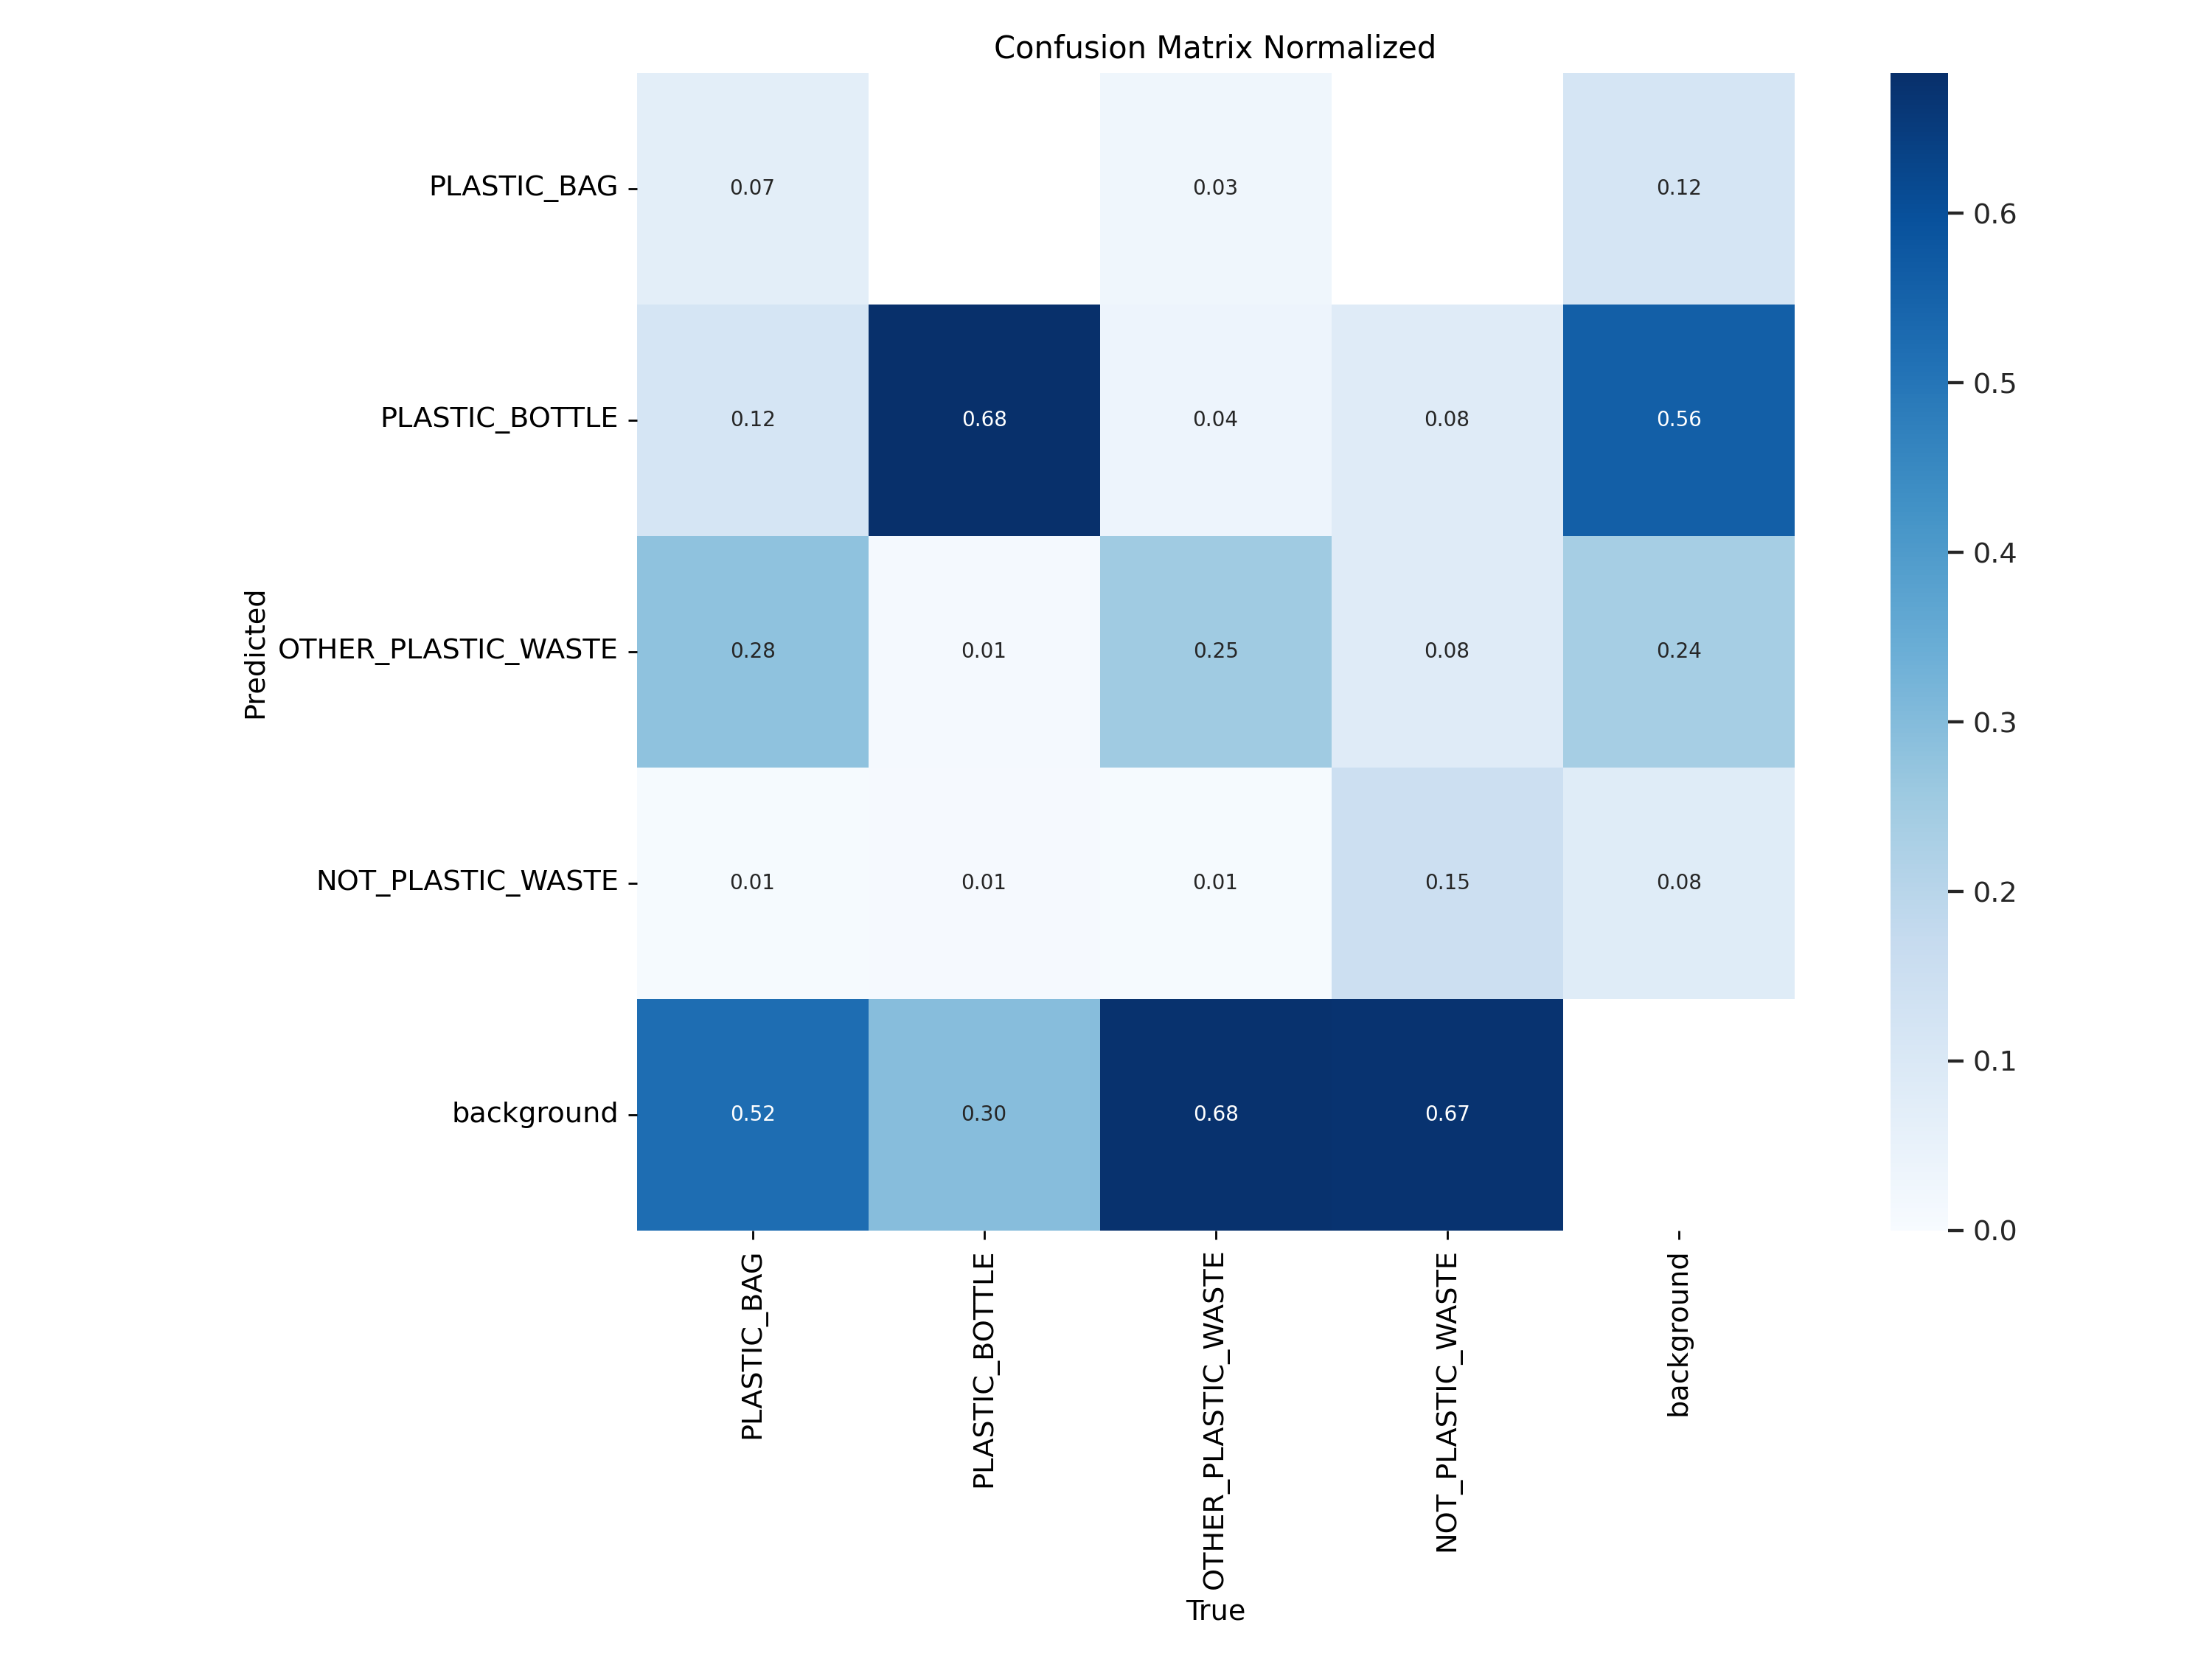
\includegraphics[width=0.8\textwidth]{v_2/small-1203/confusion_matrix_normalized.png}
    \caption{Matrice di confusione normalizzata data dal modello \texttt{small-1203}}
    \label{fig:v2-4}
\end{figure}